\section{Results and Discussion}

\definecolor{deeppeach}{rgb}{1.0, 0.8, 0.64}

\newcommand{\mcell}[1]{\makecell{~\\[-0.75cm]\makebox[0pt]{#1}}}
\newcommand{\graytext}[1]{\color{gray} #1}
\newcommand{\bluetext}[1]{\bf \cellcolor{blue!15} #1}
\newcommand{\redtext}[1]{\bf \cellcolor{red!15} #1}

% Define a new pattern for spaced crosshatches
\pgfdeclarepatternformonly{my north east lines}{\pgfqpoint{-1pt}{-1pt}}{\pgfqpoint{10pt}{10pt}}{\pgfqpoint{6pt}{6pt}}%
{
  \pgfsetlinewidth{0.4pt}
  \pgfpathmoveto{\pgfqpoint{0pt}{0pt}}
  \pgfpathlineto{\pgfqpoint{3.1pt}{3.1pt}}
  \pgfusepath{stroke}
}

\newcommand{\crosshatchedcell}[1][9pt]{%
  \begin{tikzpicture}[baseline,overlay]
    \node[anchor=south west, inner sep=0pt, outer sep=0pt, minimum width=\linewidth + 1.5em, minimum height=0.67cm, pattern=my north east lines, pattern color=black!20] at (-0.2,0) {};
  \end{tikzpicture}%
}

% \newcommand{\crosshatchedcell}{%
%   \begin{tikzpicture}[baseline,overlay]
%     \node[anchor=south west, inner sep=0pt, outer sep=0pt, minimum width=\linewidth + 1.5em, minimum height=0.67cm, pattern=north east lines, pattern color=black!20] at (-0.2,0) {};
%   \end{tikzpicture}%
% }


\newcolumntype{M}[1]{>{\centering\arraybackslash}m{#1}}
\newcolumntype{G}{>{\columncolor{deeppeach!25}\centering\arraybackslash}m{0.08\linewidth}}
\newcolumntype{S}{>{\columncolor{gray!15}\centering\arraybackslash}M{0.10\linewidth}}
\newcommand\setrowheight{\rule{0pt}{0.67cm}}
\newcolumntype{g}{>{\columncolor{gray!25}\centering\arraybackslash}c}

\begin{table*}[h!]
    \centering
    \begin{tabular}{
        c
        g
        |S||
        G
        M{0.08\linewidth}
        M{0.08\linewidth}
        M{0.08\linewidth}
        ||G
        M{0.08\linewidth}
    }
        & \rotatebox{0}{\bf \large QOS metric} &
        \rotatebox{0}{\bf \large statistic} &
        \rotatebox{60}{\textit{baseline}} &
        \rotatebox{60}{\textit{$\Rightarrow$ multithread}} &
        \rotatebox{60}{\textit{$\Rightarrow$ intranode}} &
        \rotatebox{60}{\textit{+ compute}} &
        \rotatebox{60}{\textit{baseline}} &
        \rotatebox{60}{\textit{+ faulty hw}} \\
        \hline\hline
        \setrowheight
        \multirow[b]{4}{*}{\rotatebox[origin=c]{90}{Update Period}} &
            & \mcell{median} &
            \mcell{XX ns} &
            \bluetext{\mcell{$\Delta$-XX\%}} &
            \redtext{\mcell{$\Delta$\texttt{+}XX\%}} &
            \graytext{\mcell{$\Delta$+XX\%}} &
            \mcell{2.0 ms} &
            \graytext{\mcell{$\Delta$-0.5\%}} \\ \setrowheight

        &
            & \mcell{$\sim \mathrm{MAD}$} &
            \mcell{XX\%} &
            \graytext{\mcell{XX\%}} &
            \graytext{\mcell{XX\%}} &
            \redtext{\mcell{XX\%}} &
            \mcell{3.9\%} &
            \graytext{\mcell{4.0\%}} \\ \noalign{\vskip-0.7pt} \cdashline{3-9} \noalign{\vskip0.7pt}  \setrowheight

            &
                & \crosshatchedcell\mcell{mean} &
                \crosshatchedcell\mcell{XX ns} &
                \bluetext{\crosshatchedcell\mcell{$\Delta$-XX\%}} &
                \redtext{\crosshatchedcell\mcell{$\Delta$\texttt{+}XX\%}} &
                \graytext{\crosshatchedcell\mcell{$\Delta$+XX\%}} &
                \crosshatchedcell\mcell{2.0 ms} &
                \bluetext{\crosshatchedcell\mcell{$\Delta$-0.7\%*}}  \\ \setrowheight

        & \multirow[t]{4}{*}{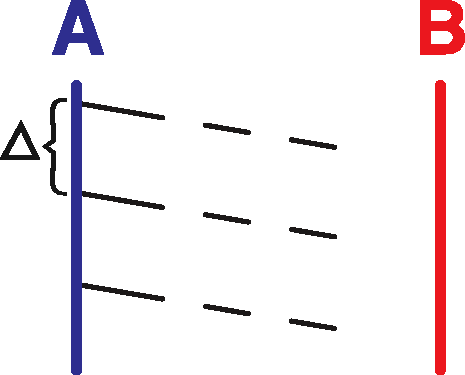
\includegraphics[height=2.8cm]{img/quality-of-service-metric-definitions/simstep-period-right.pdf}} &
            \crosshatchedcell\mcell{\% outliers} &
            \crosshatchedcell\mcell{XX\%} &
            \bluetext{\crosshatchedcell\mcell{XX\%}} &
            \graytext{\crosshatchedcell\mcell{XX\%}} &
            \graytext{\crosshatchedcell\mcell{XX\%}} &
            \crosshatchedcell\mcell{2.9\%} &
            \graytext{\crosshatchedcell\mcell{2.7\%}} \\
        \Xhline{4\arrayrulewidth}
        \setrowheight
        \multirow[t]{4}{*}{\rotatebox[origin=c]{90}{Walltime Latency~~~~~~~~~~~~~~~~~~~}} &
            & \mcell{median} &
            \mcell{XX ns} &
            \bluetext{\mcell{$\Delta$-XX\%}} &
            \redtext{\mcell{$\Delta$\texttt{+}XX\%}} &
            \graytext{\mcell{$\Delta$+XX\%}} &
            \mcell{2.3 ms} &
            \graytext{\mcell{$\Delta$-0.3\%}} \\ \setrowheight

        &
            & \mcell{$\sim \mathrm{MAD}$} &
            \mcell{XX\%} &
            \graytext{\mcell{XX\%}} &
            \graytext{\mcell{XX\%}} &
            \redtext{\mcell{XX\%}} &
            \mcell{12\%} &
            \graytext{\mcell{11\%}} \\ \noalign{\vskip-0.7pt} \cdashline{3-9} \noalign{\vskip0.7pt} \setrowheight

            &
                & \crosshatchedcell\mcell{mean} &
                \crosshatchedcell\mcell{XX ns} &
                \bluetext{\crosshatchedcell\mcell{$\Delta$-XX\%}} &
                \redtext{\crosshatchedcell\mcell{$\Delta$\texttt{+}XX\%}} &
                \graytext{\crosshatchedcell\mcell{$\Delta$+XX\%}} &
                \crosshatchedcell\mcell{2.4 ms} &
                \redtext{\crosshatchedcell\mcell{$\Delta$+446\%***}} \\ \setrowheight

        & \multirow[t]{4}{*}{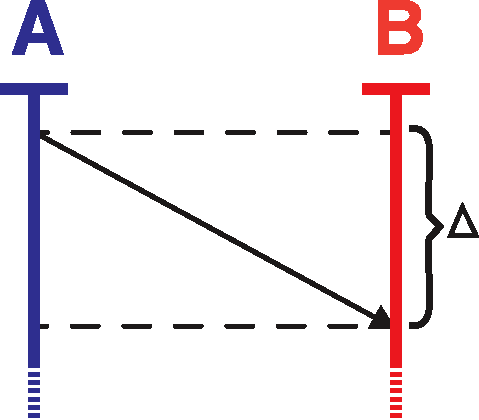
\includegraphics[height=2.8cm]{img/quality-of-service-metric-definitions/latency-right.pdf}} &
            \crosshatchedcell\mcell{\% outliers} &
            \crosshatchedcell\mcell{XX\%} &
            \bluetext{\crosshatchedcell\mcell{XX\%}} &
            \graytext{\crosshatchedcell\mcell{XX\%}} &
            \graytext{\crosshatchedcell\mcell{XX\%}} &
            \crosshatchedcell\mcell{1.8\%} &
            \graytext{\crosshatchedcell\mcell{2.1\%}} \\
        \Xhline{4\arrayrulewidth}
        \setrowheight
        \multirow[t]{4}{*}{\rotatebox[origin=c]{90}{Updates Latency~~~~~~~~~~~~~~~~~~~}} &
            & \mcell{median} &
            \mcell{XX updates} &
            \bluetext{\mcell{$\Delta$-XX\%}} &
            \redtext{\mcell{$\Delta$\texttt{+}XX\%}} &
            \graytext{\mcell{$\Delta$+XX\%}} &
            \mcell{1.2 updates} &
            \graytext{\mcell{$\Delta$+0.4\%}} \\ \setrowheight

        &
            & \mcell{$\sim \mathrm{MAD}$} &
            \mcell{XX\%} &
            \graytext{\mcell{XX\%}} &
            \graytext{\mcell{XX\%}} &
            \redtext{\mcell{XX\%}} &
            \mcell{12\%} &
            \redtext{\mcell{13\%*}} \\ \noalign{\vskip-0.7pt} \cdashline{3-9} \noalign{\vskip0.7pt} \setrowheight

            &
                & \crosshatchedcell\mcell{mean} &
                \crosshatchedcell\mcell{XX updates} &
                \bluetext{\crosshatchedcell\mcell{$\Delta$-XX\%}} &
                \redtext{\crosshatchedcell\mcell{$\Delta$\texttt{+}XX\%}} &
                \graytext{\crosshatchedcell\mcell{$\Delta$+XX\%}} &
                \crosshatchedcell\mcell{1.2 updates} &
                \redtext{\crosshatchedcell\mcell{$\Delta$+448\%***}} \\ \setrowheight

        & \multirow[t]{4}{*}{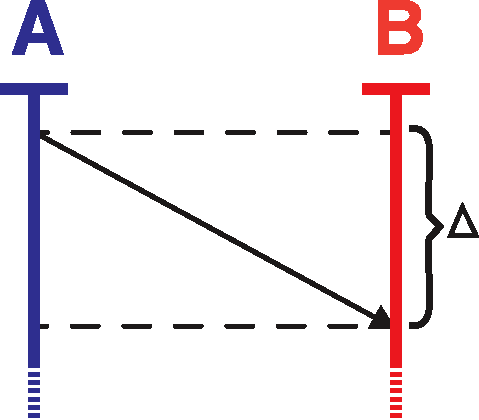
\includegraphics[height=2.8cm]{img/quality-of-service-metric-definitions/latency-right.pdf}} &
            \crosshatchedcell\mcell{\% outliers} &
            \crosshatchedcell\mcell{XX\%} &
            \bluetext{\crosshatchedcell\mcell{XX\%}} &
            \graytext{\crosshatchedcell\mcell{XX\%}} &
            \graytext{\crosshatchedcell\mcell{XX\%}} &
            \crosshatchedcell\mcell{1.9\%} &
            \redtext{\crosshatchedcell\mcell{2.3\%**}} \\
        \Xhline{4\arrayrulewidth}
        \setrowheight
        \multirow[b]{4}{*}{\rotatebox[origin=c]{90}{Bunching}} &
            & \mcell{median} &
            \mcell{XX} &
            \bluetext{\mcell{$\Delta$-XX\%}} &
            \redtext{\mcell{$\Delta$\texttt{+}XX\%}} &
            \graytext{\mcell{$\Delta$+XX\%}} &
            \mcell{0.32} &
            \graytext{\mcell{$\Delta$-0.5\%}} \\ \setrowheight

        &
            & \mcell{$\sim \mathrm{MAD}$} &
            \mcell{XX\%} &
            \graytext{\mcell{XX\%}} &
            \graytext{\mcell{XX\%}} &
            \redtext{\mcell{XX\%}} &
            \mcell{24\%} &
            \graytext{\mcell{24\%}} \\ \noalign{\vskip-0.7pt} \cdashline{3-9} \noalign{\vskip0.7pt} \setrowheight

            &
                & \crosshatchedcell\mcell{mean} &
                \crosshatchedcell\mcell{XX} &
                \bluetext{\crosshatchedcell\mcell{$\Delta$-XX\%}} &
                \redtext{\crosshatchedcell\mcell{$\Delta$\texttt{+}XX\%}} &
                \graytext{\crosshatchedcell\mcell{$\Delta$+XX\%}} &
                \crosshatchedcell\mcell{0.32} &
                \graytext{\crosshatchedcell\mcell{$\Delta$-0.6\%}} \\ \setrowheight

        & \multirow[t]{4}{*}{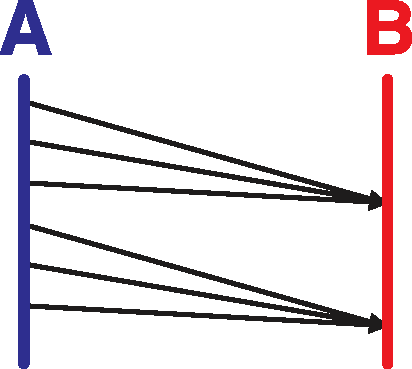
\includegraphics[height=2.8cm]{img/quality-of-service-metric-definitions/clumpiness-right.pdf}} &
            \crosshatchedcell\mcell{\% outliers} &
            \crosshatchedcell\mcell{XX\%} &
            \bluetext{\crosshatchedcell\mcell{XX\%}} &
            \graytext{\crosshatchedcell\mcell{XX\%}} &
            \graytext{\crosshatchedcell\mcell{XX\%}} &
            \crosshatchedcell\mcell{0.03\%} &
            \redtext{\crosshatchedcell\mcell{0.5\%***}} \\
        \Xhline{4\arrayrulewidth}
        \setrowheight
        \multirow[t]{4}{*}{\rotatebox[origin=c]{90}{Delivery Fail Rate~~~~~~~~~~~~~~~~~~}} &
            & \mcell{median} &
            \mcell{XX} &
            \bluetext{\mcell{$\Delta$-XX\%}} &
            \redtext{\mcell{$\Delta$\texttt{+}XX\%}} &
            \graytext{\mcell{$\Delta$+XX\%}} &
            \mcell{0} &
            \graytext{\mcell{0}} \\ \setrowheight

        &
            & \mcell{$\sim \mathrm{MAD}$} &
            \mcell{XX\%} &
            \graytext{\mcell{XX\%}} &
            \graytext{\mcell{XX\%}} &
            \redtext{\mcell{XX\%}} &
            \mcell{0\%} &
            \graytext{\mcell{0\%}} \\ \noalign{\vskip-0.7pt} \cdashline{3-9} \noalign{\vskip0.7pt} \setrowheight

            &
                & \crosshatchedcell\mcell{mean} &
                \crosshatchedcell\mcell{XX} &
                \bluetext{\crosshatchedcell\mcell{$\Delta$-XX\%}} &
                \redtext{\crosshatchedcell\mcell{$\Delta$\texttt{+}XX\%}} &
                \graytext{\crosshatchedcell\mcell{$\Delta$+XX\%}} &
                \crosshatchedcell\mcell{0} &
                \redtext{\crosshatchedcell\mcell{0.003\%**}} \\ \setrowheight

        & \multirow[t]{4}{*}{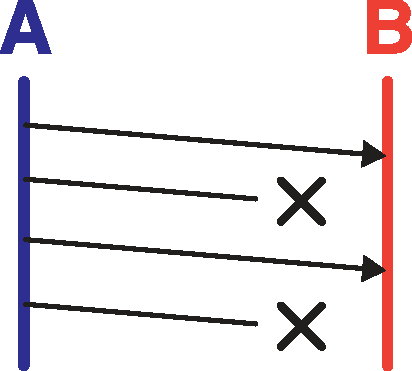
\includegraphics[height=2.8cm]{img/quality-of-service-metric-definitions/delivery-failure-rate-right.pdf}} &
            \crosshatchedcell\mcell{\% outliers} &
            \crosshatchedcell\mcell{XX\%} &
            \bluetext{\crosshatchedcell\mcell{XX\%}} &
            \graytext{\crosshatchedcell\mcell{XX\%}} &
            \graytext{\crosshatchedcell\mcell{XX\%}} &
            \crosshatchedcell\mcell{2.5\%} &
            \bluetext{\crosshatchedcell\mcell{0.7\%***}} \\
        \hline

    \end{tabular}
    \caption{%
      Best-effort communication quality of service (QOS) outcomes under experimental treatments, with 10 independent replicates per condition.
      Each QOS metric is described through four statistics.
      For each metric, the first two statistics (unhatched rows) describe typical QOS value and variance among typical QOS values.
      The second two statistics (hatched rows) describe outlier-inclusive QOS value and variance.
      Significantly degraded QOS outcomes are colored red, improved outcomes are blue, and baselines for comparison are peach.
      Significance denoted $* = p < 0.05$, $** = p < 0.005$, $*** = p < 0.0005$.
      QOS with no significant difference from baseline are grayed out.
      Statistic definitions are as follows, (1) median: median of replicate median observations, tested with quantile regression; (2) $\sim$MAD: median of relative median absolute deviance by replicate, tested with Mann-Whitney U; (3) mean: median of replicate observation means, tested with quantile regression; (4) percent outliers: percent outliers based on IQR definition, tested with chi-square contingency test.
      Values reported relative to baseline denoted $\Delta \texttt{+}x\%$ or $\Delta \texttt{-}x\%$.
    }
    \label{tab:categorical-composite}
\end{table*}


Sections \ref{sec:multithread-benchmarks} and \ref{sec:multiprocess-benchmarks} compare execution performance under the best-effort communication versus the perfect communication models.
In particular, both sections investigate how the impact of best-effort communication on performance relates to CPU count scale.
Section \ref{sec:multithread-benchmarks} covers multithreading and Section \ref{sec:multiprocess-benchmarks} covers multiprocessing.

The following sections investigate how system configuration affects quality of service.
Specifically, these sections cover the impact of
\begin{itemize}
  \item increasing compute workload per simulation update step (Section \ref{sec:computation-vs-communication}),
  \item within-node versus between-node process placement (Section \ref{sec:intranode-vs-internode}), and
  \item multithreading versus multiprocessing (Section \ref{sec:multithreading-vs-multiprocessing}).
\end{itemize}

Section \ref{sec:weak-scaling} tests how quality of service changes with CPU count.
This analysis fleshes out the performance-centric picture of best-effort scalability established in Sections \ref{sec:multithread-benchmarks} and \ref{sec:multiprocess-benchmarks}.

Section \ref{sec:with-lac-417-vs-sans-lac-417} tests how inclusion of an apparently faulty node (i.e., that provided exceptionally poor quality of service) affects global quality of service.
This experiment provides insight into the robustness of best-effort approaches to single-point failure.

\subsection{Performance: Multithread Benchmarks}

  \begin{figure}[thpb]
      \centering
    \begin{subfigure}[b]{\linewidth}
      \centering
      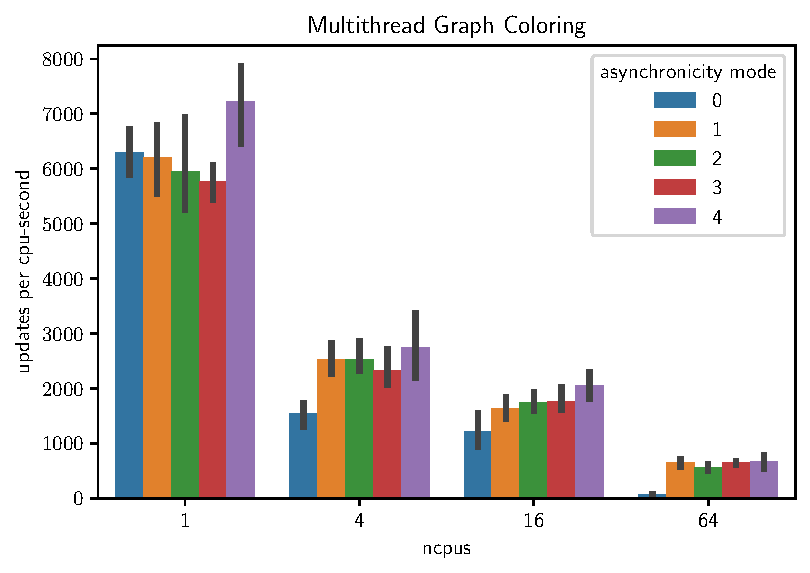
\includegraphics[width=\linewidth]{chart/multithread-graph-coloring}
     \caption{Graph coloring per-thread update rate. Higher is better.}
         \label{fig:multithread_graph_coloring_update_rate}
      \end{subfigure}
      
    \begin{subfigure}[b]{\linewidth}
      \centering
      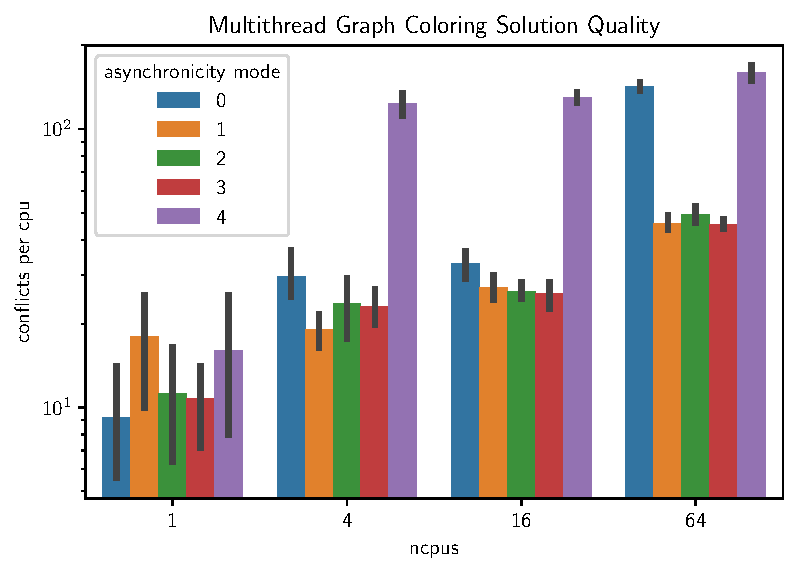
\includegraphics[width=\linewidth]{chart/multithread-graph-coloring-solution-quality}      
      \caption{Graph coloring solution conflicts. Lower is better.}
         \label{fig:multithread_graph_coloring_solution_quality}
    \end{subfigure}
    
    
    \begin{subfigure}[b]{\linewidth}
    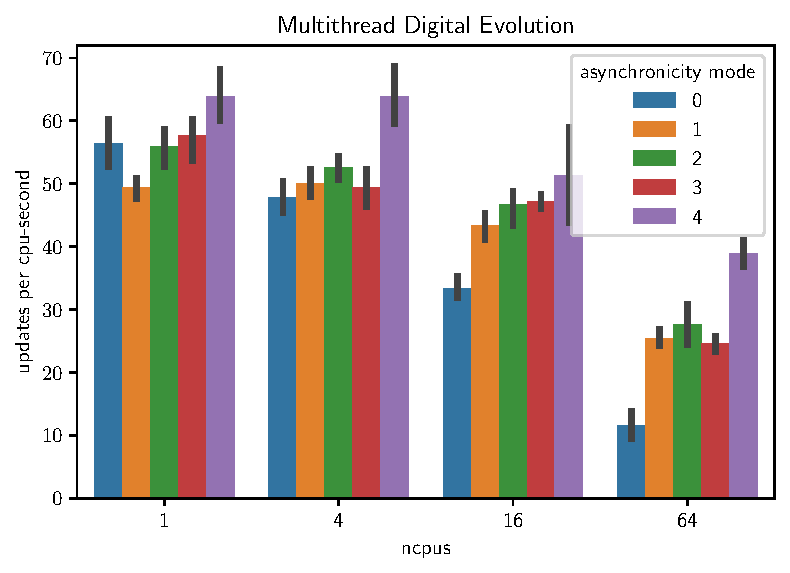
\includegraphics[width=\linewidth]{chart/multithread-digital-evolution}
    \caption{Digital evolution per-thread update rate. Higher is better.}
         \label{fig:multithread_digital_evolution_update_rate}
    \end{subfigure}

    \caption{Multithread benchmark results. Bars represent bootstrapped 95\% confidence intervals. }
      \label{fig:multithread_benchmarks}
  \end{figure}

Figure \ref{fig:multithread_graph_coloring_update_rate} presents per-cpu algorithm update rate for the graph coloring benchmark at 1, 4, 16, and 64 threads.
Update rate performance decreased with increasing multithreading across all asynchronicity modes.
This performance degradation was rather severe --- per-cpu update rate decreased by 61\% between 1 and 4 threads and by about another 75\% between 4 and 64 threads.
Surprisingly, this issue appears largely unrelated to inter-thread communication, as it was also observed in asynchronicity mode 4, where all interthread communication is disabled.
Perhaps per-cpu update rate degradation under threading was induced by strain on a limited system resource like memory cache or access to the system clock (which was used to control run timing).
This unexpectedly severe phenomenon merits further investigation to fully in future work with this benchmark.

Nevertheless, we were able to observe significantly better performance of best-effort asynchronicity modes 1, 2, and 3 at high thread counts.
At 64 threads, these run modes significantly outperformed the fully-synchronized mode 0 ($p < 0.05$, non-overlapping 95\% confidence intervals).
Likewise, as shown in Figure \ref{fig:multithread_graph_coloring_solution_quality}, best-effort asynchronicity modes were able to deliver significantly better graph coloring solutions within the allotted compute time than the fully-synchronized mode 0 ($p < 0.05$, non-overlapping 95\% confidence intervals).

Figure \ref{fig:multithread_digital_evolution_update_rate} shows per-cpu algorithm update rate for the digital evolution benchmark at 1, 4, 16, and 64 threads.
Similarly to the graph coloring benchmark, update rate performance decreased with increasing multithreading across all asynchronicity modes --- including mode 4, which eschews inter-thread communication.
Even without communication between threads, with 64 threads each thread performed updates at only 61\% the rate of a lone thread.
At 64 threads, best-effort asynchronicity modes 1, 2, and 3 exhibit about 43\% the update-rate performance of a lone thread.
Although best-effort inter-thread communication only exhibits half the update-rate performance of completely decoupled execution at 64 threads, this update-rate performance is roughly $2.1\times$ that of the fully-synchronous mode 0.
Indeed, best-effort modes significantly outperform the fully-synchronous mode on the digital evolution benchmark at both 16 and 64 threads ($p < 0.05$, non-overlapping 95\% confidence intervals).


\subsection{Performance: Multiprocess Benchmarks}

\begin{figure}[thpb]
      \centering
      
    \begin{subfigure}[b]{\linewidth}
    \centering
    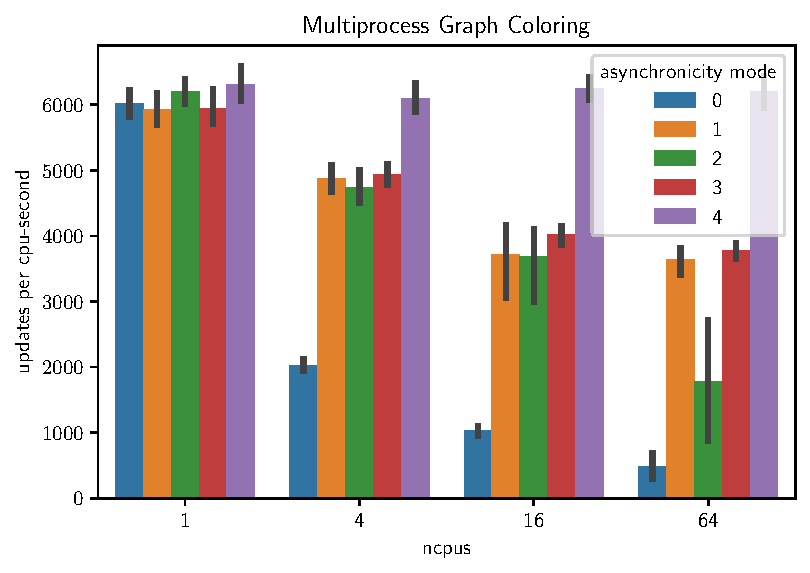
\includegraphics[width=\linewidth]{chart/multiprocess-graph-coloring}
    \caption{Graph coloring per-process update rate. Higher is better.}
    \label{fig:multiprocess_graph_coloring_update_rate}
    \end{subfigure}
    
    \begin{subfigure}[b]{\linewidth}
      \centering
      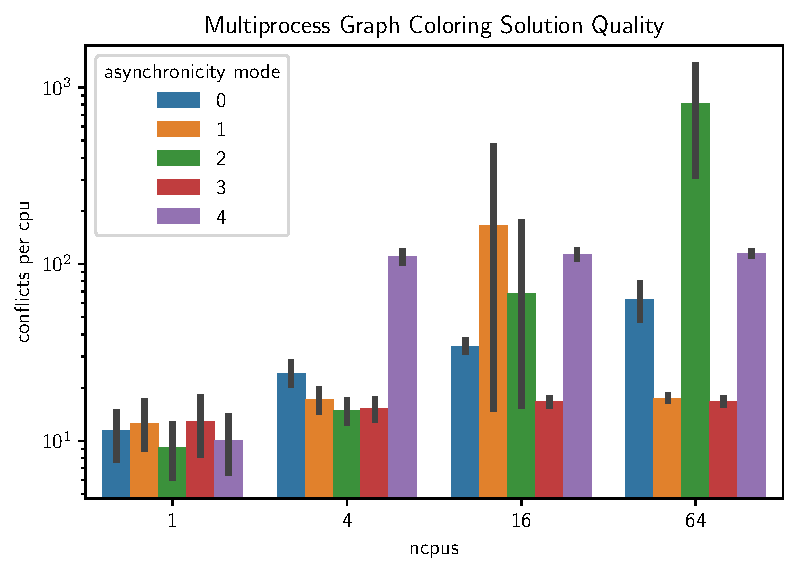
\includegraphics[width=\linewidth]{chart/multiprocess-graph-coloring-solution-quality} 
      \caption{Graph coloring solution conflicts. Lower is better.}
      \label{fig:multiprocess_graph_coloring_solution_quality}
    \end{subfigure}

  \begin{subfigure}[b]{\linewidth}
    \centering
  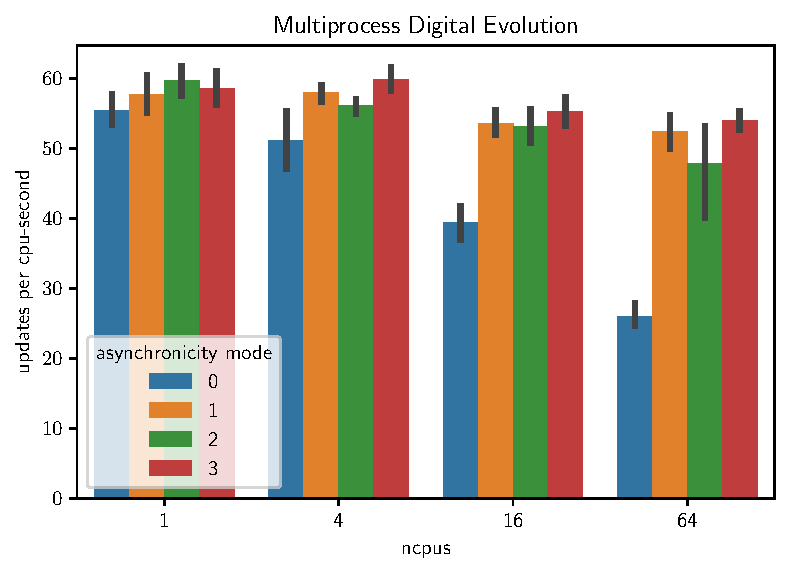
\includegraphics[width=\linewidth]{chart/multiprocess-digital-evolution}
  \caption{Digital evolution per-process update rate. Higher is better.}
  \label{fig:multiprocess_digital_evolution_update_rate}
  \end{subfigure}
      
  \caption{Multiprocess benchmark results. Bars represent bootstrapped 95\% confidence intervals. }
  \label{fig:multiprocess_benchmarks}
\end{figure}

Figure \ref{fig:multiprocess_graph_coloring_update_rate} shows per-cpu algorithm update rate for the graph coloring benchmark at 1, 4, 16, and 64 processes.
Unlike the multithreaded benchmark, multiprocess graph coloring exhibits consistent update-rate performance across process counts under asynchronicity mode 4, where inter-thread communication is disabled.
This matches the expectation that, indeed, with comparable hardware a single process should exhibit the same mean performance as any number of completely decoupled processes.
At 64 processes, best-effort asynchronicity mode 3 exhibits about 63\% the update-rate performance of single-process execution.
This represents about an $7.8\times$ speedup compared to fully-synchronous mode 0.
Indeed, best-effort mode 3 enables significantly better per-cpu update rates at 4, 16, and 64 processes ($p < 0.05$, non-overlapping 95\% confidence intervals).

Likewise, shown in Figure \ref{fig:multiprocess_graph_coloring_solution_quality}, best-effort asynchronicity mode 3 yields significantly better graph-coloring results within the allotted time at 4, 16, and 64 processes ($p < 0.05$, non-overlapping 95\% confidence intervals).
Interestingly, partial-synchronization modes 1 and 2 exhibited highly inconsistent solution quality performance at 16 and 64 process count benchmarks.
Fixed-timepoint barrier sync (mode 2) had particularly poor performance performance at 64 processes (note the log-scale axis).
We suspect this was caused by a race condition where workers would assign sync points to different fixed points different based on slightly different startup times (i.e., process 0 syncs at seconds 0, 1, 2... while process 1 syncs at seconds 1, 2, 3..).

Figure \ref{fig:multiprocess_digital_evolution_update_rate} presents per-cpu algorithm update rate for the digital evolution benchmark at 1, 4, 16, and 64 processes.
Relative performance fares well at high process counts under this relatively computation-heavy workload, with 64-process fully best-effort simulation exhibiting about 92\% the update rate of single-process simulation.
This represents a $2.1\times$ speedup compared to the fully-synchronous run mode 0.
Best-effort significantly mode 3 outperforms the per-cpu update rate of fully-synchronous mode 0 at process counts 16 and 64 ($p < 0.05$, non-overlapping 95\% confidence intervals).


\subsection{Quality of Service: Computation vs. Communication}

Having shown performance benefits of best-effort communication on the graph coloring and digital evolution benchmarks in Sections \ref{sec:multithread-benchmarks} and \ref{sec:multiprocess-benchmarks}, we next seek to more fully characterize the best-effort approach using a holistic suite of proposed quality of service metrics.
This section evaluates how a simulation's ratio of communication intensity to computational work affects these quality of service metrics.
The graph coloring benchmark serves as our experimental system.

For this experiment, arbitrary compute work (detached from the underlying algorithm) was added to the simulation update process.
We used a call to the \texttt{std::mt19937} random number engine as a unit of compute work.
In microbenchmarks, we found that one work unit consumed about 35ns of walltime and 21ns of compute time.
We performed 5 treatments, adding \numprint{0}, \numprint{64}, \numprint{4096}, \numprint{262144}, or \numprint{16777216} units of compute work to the update process.
For each treatment, measurements were made on a pair of processes split across different nodes within the same cluster.

\subsubsection{Simstep Period}

Unsurprisingly, we found a direct relationship between per-update computational workload and the walltime required per computational update.
Supplementary Figures \ref{fig:computation-vs-communication-distribution-simstep-period-inlet-ns} and \ref{fig:computation-vs-communication-distribution-simstep-period-outlet-ns} depict the distribution of walltime per computational update across snapshots.
Once added compute work supersedes the light compute work already associated with the graph coloring algorithm update step (at around 64 work units), simstep period appears to scale in direct proportion with compute work.
Indeed, we found a significant positive relationship between both mean and median simstep period and added compute work (Supplementary Figures \ref{fig:computation-vs-communication-regression-simstep-period-inlet-ns} and \ref{fig:computation-vs-communication-regression-simstep-period-outlet-ns}).
At 0 units of added compute work, mean and median simstep period was 14.7 \SI{14.7}{\micro\second} (both inlet/outlet).
At \numprint{16777216} units of added compute work, mean simstep period was 614ms inlet/608ms outlet and median simstep period was 506ms inlet/508ms outlet.
Supplementary Tables \ref{tab:computation-vs-communication-ordinary-least-squares-regression} and \ref{tab:computation-vs-communication-quantile-regression} detail numerical results of these regressions.

\subsubsection{Simstep Latency}

Unsurprisingly, again, we observed a negative relationship between the number of simulation steps elapsed during message transit and added computational work.
Put simply, longer update steps provide more time for messages to transit.
Supplementary Figures \ref{fig:computation-vs-communication-distribution-latency-simsteps-inlet} and \ref{fig:computation-vs-communication-distribution-latency-simsteps-outlet} show the distribution of simstep latency across compute workloads.
With no added compute work, messages take between 20 and 100 simulation steps to transit (mean: 48.2 updates inlet/47.9 updates outlet; median: 42.5 updates inlet/outlet).
At maximum compute work per update, messages arrive at a median 1.00 update latency.
Regression analysis confirms a significant negative relationship between both mean and median log simstep latency and log added compute work (Supplementary Figures \ref{fig:computation-vs-communication-regression-latency-simsteps-inlet} and \ref{fig:computation-vs-communication-regression-latency-simsteps-outlet}).
Supplementary Tables \ref{tab:computation-vs-communication-ordinary-least-squares-regression} and \ref{tab:computation-vs-communication-quantile-regression} detail numerical results of these regressions.

%TODO use log latency simsteps for estimated statistics --- regressions are broken for raw input

\subsubsection{Walltime Latency}

Effects of log compute work on our measure of walltime latency highlight an important caveat in the interpretation of this metric.
At \numprint{0}, \numprint{64}, and \numprint{4096} work units, walltime latency measures $\approx 1$ ms (means: \SI{710}{\micro\second}, \SI{794}{\micro\second}, \SI{906}{\micro\second} inlet / \SI{706}{\micro\second}, \SI{782}{\micro\second}, \SI{899}{\micro\second}; medians: \SI{623}{\micro\second}, \SI{639}{\micro\second}, \SI{742}{\micro\second} inlet / \SI{622}{\micro\second}, \SI{642}{\micro\second}, \SI{733}{\micro\second} outlet).
However, once simstep period grows to $\approx 10$ ms at \numprint{262144} work units and (an order of magnitude in excess of walltime latency observed at low compute loads), walltime latency increases with added compute work.
At \numprint{16777216} compute work units, 1.00s inlet / 1.01s outlet median walltime latency is observed.
Because our computational model assumes on-demand message delivery with a communication phase only occurring once per simulation update, message transmission speed is fundamentally limited by simulation update period.
If a message is dispatched while its recipient is busy doing computational work, the soonest it can be received will be when that recipient completes the computational phase of its update.
In order to measure transmission time fully independent of delays due to on-demand delivery, additional instrumentation would be necessary.
However, when this latency is greater than a few simsteps, this measure is reasonably representative of message transmission time.

Supplementary Figures \ref{fig:computation-vs-communication-distribution-latency-walltime-inlet-ns} and \ref{fig:computation-vs-communication-distribution-latency-walltime-outlet-ns} show the distribution of walltime latency across computational workloads.
Supplementary Figures \ref{fig:computation-vs-communication-regression-latency-walltime-inlet-ns} and \ref{fig:computation-vs-communication-regression-latency-walltime-outlet-ns} summarize regression between walltime latency and added compute work.
Supplementary Tables \ref{tab:computation-vs-communication-ordinary-least-squares-regression} and \ref{tab:computation-vs-communication-quantile-regression} detail numerical results of those regressions.

\subsubsection{Delivery Clumpiness}

We observed a negative relationship between computation workload and delivery clumpiness.
At low computational intensity, we observed clumpiness greater than 0.95, meaning that fewer than 5\% of pull requests were laden with fresh messages (at 0 compute work mean: 0.96, median 0.96).
However, at high computational intensity clumpiness reached 0, indicating that messages arrived as a steady stream (at \numprint{16777216} compute work mean: 0.00, median 0.00).
Ostensibly, the reduction in clumpiness is due to increased real-time separation between dispatched messages.
Supplementary Figure \ref{fig:computation-vs-communication-distribution-delivery-clumpiness} shows the effect of computational workload on the distribution of observed clumpinesses.
We found a significant negative relationship between both mean and median clumpiness and computational intensity.
Supplementary Figure \ref{fig:computation-vs-communication-regression-delivery-clumpiness} visualizes these regressions and Supplementary Tables \ref{tab:computation-vs-communication-ordinary-least-squares-regression} and \ref{tab:computation-vs-communication-quantile-regression} provide numerical details.

\subsubsection{Delivery Failure Rate}

We did not observe any delivery failures across all replicates and all compute workloads.
So, compute workload had no observable effect on delivery reliability.
Interestingly, as discussed in Section \ref{sec:intranode-vs-internode}, we did observe some delivery failure under intranode conditions.
However, these experiments were conducted under internode conditions.
Supplementary Figure \ref{fig:computation-vs-communication-distribution-delivery-failure-rate} shows the distribution of delivery failure rates across computation workloads and Supplementary Figure \ref{fig:computation-vs-communication-regression-delivery-failure-rate} shows regressions of delivery failure rate of against computational workload
See Supplementary Tables \ref{tab:computation-vs-communication-ordinary-least-squares-regression} and \ref{tab:computation-vs-communication-quantile-regression} for numerical details.


\subsection{Quality of Service: Intranode vs. Internode}
\label{sec:intranode-vs-internode}

This section tests the effect of process assignment on best-effort quality of service, comparing multi-node and single-node assignments.
The graph coloring benchmark again serves as our experimental substrate.

For this experiment, processes were either assigned to the same node or were assigned to different nodes.
In both cases, we used two processes.

\subsubsection{Simstep Period}

Simstep period was significantly slower under internode conditions than under intranode conditions.

% When processes shared the same node, simstep period was around \SI{9}{\micro\second} (mean: \SI{9.07}{\micro\second} inlet / \SI{9.04}{\micro\second} outlet; median: \SI{9.11}{\micro\second} inlet / \SI{9.05}{\micro\second}).
When processes shared the same node, simstep period was around \SI{9}{\micro\second} (mean: \SI{9.06}{\micro\second}; median: \SI{9.08}{\micro\second}).
% Under internode conditions, simstep period was around \SI{14}{\micro\second} (mean: \SI{14.5}{\micro\second} inlet/outlet; median: \SI{14.5}{\micro\second} inlet / \SI{14.4}{\micro\second} outlet).
Under internode conditions, simstep period was around \SI{14}{\micro\second} (mean: \SI{14.5}{\micro\second}; median: \SI{14.4}{\micro\second}).
Supplementary Figures \ref{fig:intranode-vs-internode-distribution-simstep-period-inlet-ns} and \ref{fig:intranode-vs-internode-distribution-simstep-period-outlet-ns} depict the distribution of walltime per computational update across intranode and internode conditions.

This result presumably attributes to an increased walltime cost for calls to the MPI implementation backing internode communication compared to the MPI implementation backing intranode communication.
Although this effect is clearly detectable, its magnitude is modest given the minimal computational intensity of the simulation update step --- only $\approx 56\%$ more expensive than intranode dispatch.

Both mean and median simstep period increased significantly under internode conditions.
(Supplementary Figures \ref{fig:intranode-vs-internode-regression-simstep-period-inlet-ns} and \ref{fig:intranode-vs-internode-regression-simstep-period-outlet-ns} visualize these regressions and Supplementary Tables \ref{tab:intranode-vs-internode-ordinary-least-squares-regression} and \ref{tab:intranode-vs-internode-quantile-regression} detail numerical results.)

\subsubsection{Simstep Latency}

Significantly more simulation updates transpired during message transmission under internode condtions compared to intranode conditions.

Supplementary Figures \ref{fig:intranode-vs-internode-distribution-latency-simsteps-inlet} and \ref{fig:intranode-vs-internode-distribution-latency-simsteps-outlet} compares the distributions of simstep latency across these conditions.
% Simstep latency was around 1 update for intranode communication (mean: 1.01 updates inlet / 0.99 updates outlet; median 0.75 updates inlet / outlet) and around 40 updates for internode communication (mean: 41.8 updates inlet / 41.4 updates outlet; median: 37.4 updates inlet / outlet).
Simstep latency was around 1 update for intranode communication (mean: 1.00 updates; median 0.75 updates) and around 40 updates for internode communication (mean: 41.6 updates; median: 37.4 updates).

Regression analysis confirms the significant effect of process placement on simstep latency (Supplementary Figures \ref{fig:intranode-vs-internode-regression-latency-simsteps-inlet} and \ref{fig:intranode-vs-internode-regression-latency-simsteps-outlet}).
Supplementary Tables \ref{tab:intranode-vs-internode-ordinary-least-squares-regression} and \ref{tab:intranode-vs-internode-quantile-regression} detail numerical results of these regressions.

\subsubsection{Walltime Latency}

Significantly more walltime elapsed during message transmission under internode condtions compared to intranode conditions.

% Walltime latency was less than \SI{10}{\micro\second} for intranode communication (mean: \SI{7.72}{\micro\second} inlet / \SI{7.69}{\micro\second}; median: \SI{6.95}{\micro\second} inlet / \SI{6.93}{\micro\second}).
Walltime latency was less than \SI{10}{\micro\second} for intranode communication (mean: \SI{7.70}{\micro\second}; median: \SI{6.94}{\micro\second}).
% Internode communication had approximately $50\times$ greater walltime latency, at around \SI{500}{\micro\second} (mean: \SI{604}{\micro\second} inlet / \SI{596}{\micro\second} outlet; median: \SI{554}{\micro\second} inlet / \SI{548}{\micro\second} outlet).
Internode communication had approximately $50\times$ greater walltime latency, at around \SI{500}{\micro\second} (mean: \SI{600}{\micro\second}; median: \SI{551}{\micro\second}).

Supplementary Figures \ref{fig:intranode-vs-internode-distribution-latency-walltime-inlet-ns} and \ref{fig:intranode-vs-internode-distribution-latency-walltime-outlet-ns} show the distributions of walltime latency for intra- and inter-node communication.
Regression analysis confirmed a significant increase in walltime latency under inter-node communication (Supplementary Figures \ref{fig:intranode-vs-internode-regression-latency-walltime-inlet-ns}, \ref{fig:intranode-vs-internode-regression-latency-walltime-outlet-ns}; Supplementary Tables \ref{tab:intranode-vs-internode-ordinary-least-squares-regression} and \ref{tab:intranode-vs-internode-quantile-regression}).

\subsubsection{Delivery Clumpiness}

Delivery clumpiness was minimal under intranode communication and very high under internode communication.

Under intranode conditions, we observed a mean clumpiness value of 0.014 and a median of 0.002.
Under internode conditions, we observed mean and median clumpiness values of 0.96.
Supplementary Figures \ref{fig:intranode-vs-internode-distribution-delivery-clumpiness} and \ref{fig:intranode-vs-internode-distribution-delivery-clumpiness} show the distributions of clumpiness for intra- and inter-node communication.
Regression analysis confirmed a significant increase in clumpiness under inter-node communication (Supplementary Figures \ref{fig:intranode-vs-internode-regression-delivery-clumpiness}, \ref{fig:intranode-vs-internode-regression-delivery-clumpiness}; Supplementary Tables \ref{tab:intranode-vs-internode-ordinary-least-squares-regression} and \ref{tab:intranode-vs-internode-quantile-regression}).

\subsubsection{Delivery Failure Rate}

Somewhat counterintuitively, a significantly higher proportion of deliveries failed for intranode communication than for internode communication.

We observed a delivery failure rate of around 0.3 for intranode communication (mean: 0.33; median: 0.30) and no delivery failures for internode communication (mean: 0.00; median: 0.00).
In some intranode snapshot windows, we observed a delivery failure rate as high as 0.8.
Supplementary Figures \ref{fig:intranode-vs-internode-distribution-delivery-clumpiness} and \ref{fig:intranode-vs-internode-distribution-delivery-clumpiness} show the distributions of delivery failure rate for intra- and inter-node communication.

Because of Conduit's current MPI-based implementation, messages only drop when the underlying send buffer fills; queued messages are guaranteed for delivery.
Slower simstep period under internode allocation could improve stability of the send buffer due to more time, on average, between send attempts.
Underlying buffering or consolidation by the MPI backend for internode communication might also play a role by allowing data to be moved out of the userspace send buffer more promptly.

Regression analysis confirmed a significant increase in delivery failure under intra-node communication (Supplementary Figures \ref{fig:intranode-vs-internode-regression-delivery-clumpiness}, \ref{fig:intranode-vs-internode-regression-delivery-clumpiness}; Supplementary Tables \ref{tab:intranode-vs-internode-ordinary-least-squares-regression} and \ref{tab:intranode-vs-internode-quantile-regression}).


\subsection{Quality of Service: Multithreading vs. Multiprocessing}
\label{sec:multithreading-vs-multiprocessing}

This section compares best-effort quality of service under multithreading and multiprocessing schemes.
We hold hardware configuration constant by restricting multiprocessing to cores a single hardware node, as is the case for multithreading.
However, inter-process communication occurred via MPI calls while inter-thread communication occurring via shared memory access mediated by a C++ \texttt{std::mutex}.

The graph coloring benchmark again serves as our experimental system.
Both treatments used a single pair of CPUs.

\subsubsection{Simstep Period}

Multithreading enabled faster simulation update turnover than multiprocessing.

Under multithreading, simstep period was around \SI{5}{\micro\second} (mean: \SI{4.62}{\micro\second} inlet / \SI{4.60}{\micro\second} outlet; median: \SI{4.64}{\micro\second} inlet / outlet).
Simstep period for multiprocessing was around \SI{9}{\micro\second} (mean: \SI{9.01}{\micro\second} inlet / \SI{8.98}{\micro\second} outlet; median: \SI{9.07}{\micro\second} inlet / \SI{9.01}{\micro\second} outlet).
Supplementary Figures \ref{fig:multithreading-vs-multiprocessing-distribution-simstep-period-inlet-ns} and \ref{fig:multithreading-vs-multiprocessing-distribution-simstep-period-outlet-ns} depict the distribution of walltime per computational update for both multiprocessing and multithreading.
This result falls in line with expectations that interaction via shared memory incurs lower overhead than via MPI calls.

Regression analysis showed that both mean and median simstep period were significantly slower under multiprocessing compared to multithreading.
(Supplementary Figures \ref{fig:multithreading-vs-multiprocessing-regression-simstep-period-inlet-ns} and \ref{fig:multithreading-vs-multiprocessing-regression-simstep-period-outlet-ns} visualize these regressions and Supplementary Tables \ref{tab:multithreading-vs-multiprocessing-ordinary-least-squares-regression} and \ref{tab:multithreading-vs-multiprocessing-quantile-regression} detail numerical results.)

\subsubsection{Walltime Latency}

No significant difference in walltime latency was detected between multiprocessing and multithreading.

In the median case, walltime latency was approximately \SI{5}{\micro\second} for multithreading (\SI{5.05}{\micro\second} inlet / \SI{5.08}{\micro\second} outlet) and \SI{8}{\micro\second} for multiprocessing (\SI{7.84}{\micro\second} inlet / \SI{7.80}{\micro\second} outlet).
However, a pair of extreme outliers among snapshot windows --- with walltime latencies of approximately 12ms --- drove multithreading walltime latency much higher in the mean case (\SI{448}{\micro\second} inlet / \SI{454}{\micro\second} outlet).
In the mean case, multiprocessing walltime latency was \SI{8.65}{\micro\second} inlet / \SI{8.48}{\micro\second} outlet.

Cache invalidation or mutex contention provide possible explanations for the observed episodes of extreme multithreading latency, although magnitude on the order of milliseconds for such effects is surprising.
Multithreading appears to provide marginally lower latency service in the median case, but at the cost of vulnerability to extreme high-latency disruptions.

Supplementary Figures \ref{fig:multithreading-vs-multiprocessing-distribution-latency-walltime-inlet-ns} and \ref{fig:multithreading-vs-multiprocessing-distribution-latency-walltime-outlet-ns} show the distributions of walltime latency for multithread and multiprocess runs.
Regression analysis did not detect any significant difference in walltime latency between multithreading and multiprocessing (Supplementary Figures \ref{fig:multithreading-vs-multiprocessing-regression-latency-walltime-inlet-ns}, \ref{fig:multithreading-vs-multiprocessing-regression-latency-walltime-outlet-ns}; Supplementary Tables \ref{tab:multithreading-vs-multiprocessing-ordinary-least-squares-regression} and \ref{tab:multithreading-vs-multiprocessing-quantile-regression}).

\subsubsection{Simstep Latency}

No significant difference in simstep latency was detected between multiprocessing and multithreading.

In the median case, multiprocessing offered marginally lower simstep latency than multithreading.
Median simstep latency was 0.84 updates inlet/outlet under multiprocessing and 1.10 updates inlet / 1.11 updates outlet under multithreading.
However, just as for walltime latency, extreme magintude outliers ($\approx$ \numprint{2000} simsteps) boosted mean simstep latency for multithreading.
Mean simstep latency was 0.95 updates inlet / 0.94 updates outlet under multiprocessing and 77.0 updates inlet / 78.0 updates outlet under multithreading.
Supplementary Figures \ref{fig:multithreading-vs-multiprocessing-distribution-latency-simsteps-inlet} and \ref{fig:multithreading-vs-multiprocessing-distribution-latency-simsteps-outlet} compare the distributions of simstep latency across these conditions.

Direct measurements of simstep period and walltime latency suggest that faster simstep period, rather than slower walltime latency, explain the marginally higher simstep latency under multithreading.

Regression analysis detected no significant effect of threading versus processing on simstep latency in both the mean and median cases (Supplementary Figures \ref{fig:multithreading-vs-multiprocessing-regression-latency-simsteps-inlet} and \ref{fig:multithreading-vs-multiprocessing-regression-latency-simsteps-outlet}).
Supplementary Tables \ref{tab:multithreading-vs-multiprocessing-ordinary-least-squares-regression} and \ref{tab:multithreading-vs-multiprocessing-quantile-regression} detail numerical results of these regressions.

\subsubsection{Delivery Clumpiness}

Multithreading exhibited higher median clumpiness and greater variance in clumpiness than multiprocessing.

Under multithreading, clumpiness was nearly 1 within some snapshot windows and less than 0.1 within others.
Under multiprocessing, clumpiness was consistently less than 0.1.
Supplementary Figures \ref{fig:multithreading-vs-multiprocessing-distribution-delivery-clumpiness} and \ref{fig:multithreading-vs-multiprocessing-distribution-delivery-clumpiness} show the distributions of clumpiness under both multiprocessing and multithreading.
Multithreading median clumpiness was 0.54.
Multiprocessing median clumpiness was 0.03.
Multithreading and multiprocessing mean clumpinesses were 0.56 and 0.03, respectively.

Regression analysis confirmed a significantly greater clumpiness under both multithreading compared to multiprocessing (Supplementary Figures \ref{fig:multithreading-vs-multiprocessing-regression-delivery-clumpiness}, \ref{fig:multithreading-vs-multiprocessing-regression-delivery-clumpiness}; Supplementary Tables \ref{tab:multithreading-vs-multiprocessing-ordinary-least-squares-regression} and \ref{tab:multithreading-vs-multiprocessing-quantile-regression}).
This result falls in line with other results suggesting that multithreading providing less consistent quality of service than multiprocessing.

\subsubsection{Delivery Failure Rate}

We observed a higher proportion of deliveries fail for multiprocessing than for multithreading.
(This is as expected; the multithread implementation directly wrote updates to a piece of shared memory, so there was no send buffer to backlog and induce message drops.)

Multiprocessing exhibited both mean and median delivery failure rate of 0.38.
In individual multiprocessing snapshot windows, we observed a delivery failure rates ranging from less than 0.1 to as high as 0.7.
We observed no multithreaded delivery failures.
Supplementary Figures \ref{fig:multithreading-vs-multiprocessing-distribution-delivery-clumpiness} and \ref{fig:multithreading-vs-multiprocessing-distribution-delivery-clumpiness} show the distributions of delivery failure rate for multithreading and multiprocessing.

Regression analysis confirmed a significant increase in delivery failure under multiprocessing (Supplementary Figures \ref{fig:multithreading-vs-multiprocessing-regression-delivery-clumpiness}, \ref{fig:multithreading-vs-multiprocessing-regression-delivery-clumpiness}; Supplementary Tables \ref{tab:multithreading-vs-multiprocessing-ordinary-least-squares-regression} and \ref{tab:multithreading-vs-multiprocessing-quantile-regression}).


\subsection{Quality of Service: Weak Scaling} \label{sec:weak-scaling}

Sections \ref{sec:multiprocess-benchmarks} and \ref{sec:multithread-benchmarks} showed how best-effort communication could improve application performance, particularly when scaling up processor count.
Performance exhibited promising properties under multiprocess scaling, with overlapping performance estimate intervals for 16 and 64 processor counts on both surveyed benchmark problems.
This section aims to flesh out how increasing processor count affects a comprehensive suite of quality of service metrics.
Our particular interest is in which, if any, aspects of quality of service degrade under larger processing pools.

To address these questions, we performed weak scaling experiments on 16, 64, and 256 processes using the graph coloring benchmark.
To broaden the survey, we tested scaling under four treatments from the Cartesian product of two variables: processors allocated per node and simulation elements assigned per processor.
For the first variable, we tested scaling on allocations with each processor hosted on an independent node and allocations where each node hosted an average of four processors.
This allowed us to examine how quality of service fared in homogeneous network conditions, where all communication between processes was inter-node, compared to heteregeneous conditions, where some inter-process communication was inter-node and some was intra-node.
For the second variable, we tested with 2'048 simulation elements (``simels'') per processor (consistent with the benchmarking experiments performed in Sections \ref{sec:multiprocess-benchmarks} and \ref{sec:multithreading-benchmarks}) and just one simulation element per processor, maximizing communication relative to computation.

\subsubsection{Simstep Period}

Supplementary Figures \ref{fig:weak-scaling-distribution-simstep-period-inlet-ns} and \ref{fig:weak-scaling-distribution-simstep-period-outlet-ns} survey the distributions of simstep periods observed within snapshot windows.
Simstep period registers around \SI{80}{\micro\second} with one simel and around \SI{200}{\micro\second} with 2'048 simels.
However, on heterogeneous allocations (4 cpus per node) this metric is more variable, spanning up to an order of magnitude.
Outlier observations range up to around 10ms with 2'048 simels and up to slightly less than 100ms inlet / 4s outlet with 1 simel.

We performed an ordinary least squares (OLS) regression to test how mean simstep period changed with processor count.
In all cases except one simel per cpu with four cpus per node, mean simstep period increased significantly with processor count from 16 to 64 to 256.
However, from 64 to 256 processors mean simstep period only increased significantly with one simel per cpu and one cpu per node.
Between 64 and 256 processes, mean simstep period actually decreased significantly for runs with 2'048 simels per cpu.
Supplementary Figures \ref{fig:weak-scaling-regression-ols-simstep-period-inlet-ns} and \ref{fig:weak-scaling-regression-ols-simstep-period-outlet-ns} visualize reported OLS regressions.
Supplementary Tables \ref{tab:weak-scaling-simstep-period-inlet-ns-regression-ols} and \ref{tab:weak-scaling-simstep-period-outlet-ns-regression-ols} provide numerical details on reported OLS regressions.

Median simstep period exhibited the same relationships with processor count, tested with quartile regression.
Supplementary Figures \ref{fig:weak-scaling-regression-quantile-simstep-period-inlet-ns} and \ref{fig:weak-scaling-regression-quantile-simstep-period-outlet-ns} visualize corresponding quartile regressions.
Supplementary Tables \ref{tab:weak-scaling-simstep-period-inlet-ns-regression-quantile} and \ref{tab:weak-scaling-simstep-period-outlet-ns-regression-quantile} report numerical details on those quartile regressions.

\subsubsection{Walltime Latency}

Walltime latency sits at around \SI{500}{\micro\second} for one-simel runs and around 2ms for 2'048-simel runs.
However, variability is greater for heterogeneous (four cpus per node) allocations.
Extreme outliers of up to almost 100ms inlet/2s outlet occur in four cpus per node, one-simel runs.
In 256 process, 2'048-simel, one cpu per node runs, outliers of more than 10s occur.
Supplementary Figures \ref{fig:weak-scaling-distribution-latency-walltime-inlet-ns} and \ref{fig:weak-scaling-distribution-latency-walltime-outlet-ns} show the distribution of walltime latencies observed across run conditions.

We performed OLS regressions to test how mean walltime latency changed with processor count.
Over 16, 64, and 256 processes, mean walltime latency increased significantly with processor count only with 2'048 simels per cpu.
Between 64 and 256 processes, mean walltime latency increased significantly with processor count only for one cpu per node with 2'048 simels per cpu.
Supplementary Figures \ref{fig:weak-scaling-regression-ols-latency-walltime-inlet-ns} and \ref{fig:weak-scaling-regression-ols-latency-walltime-outlet-ns} show these regressions.
Supplementary Tables \ref{tab:weak-scaling-latency-walltime-inlet-ns-regression-ols} and \ref{tab:weak-scaling-latency-walltime-outlet-ns-regression-ols} provide numerical details.

Next, we performed quantile regressions to test how processor count affected median walltime latency.
Over 16, 64, and 256 processes, median walltime latency increased significantly only with 4 cpus per node and 2'048 simels per cpu.
Over 64 and 256 processes, there was no significant relationship between processor count and median walltime latency under any condition.
Supplementary Figures \ref{fig:weak-scaling-regression-quantile-latency-walltime-inlet-ns} and \ref{fig:weak-scaling-regression-quantile-latency-walltime-outlet-ns} show regressions performed.
Supplementary Tables \ref{tab:weak-scaling-latency-walltime-inlet-ns-regression-quantile} \ref{tab:weak-scaling-latency-walltime-outlet-ns-regression-quantile} provide numerical details.

\subsubsection{Simstep Latency}

Simstep latency sits around 7 updates for runs with one simel per cpu and around 1.2 updates for runs with 2'048 simels per cpu.
For runs with one simel per cpu, outlier snapshot windows reach up to 50 updates underhomogeneous allocations and up to almost 100 updates under heterogeneous allocations.
The 2'048 simels per cpu, one cpu per node, 256 process condition exhibited outliers of up to almost 8'000 update simstep latency.
Supplementary Figures \ref{fig:weak-scaling-distribution-latency-simsteps-inlet} and \ref{fig:weak-scaling-distribution-latency-simsteps-outlet}  show the distribution of simstep latencies observed across run conditions.

Over 16, 64, and 256 processes, mean simstep latency increased with process count only under 1 cpu per node, 2'048 simel per cpu conditions.
The same was true over just 64 to 256 processes.
Supplementary Figures \ref{fig:weak-scaling-regression-ols-latency-simsteps-inlet} and \ref{fig:weak-scaling-regression-ols-latency-simsteps-outlet} show the OLS regressions performed, with
Supplementary Tables \ref{tab:weak-scaling-latency-simsteps-inlet-regression-ols} and \ref{tab:weak-scaling-latency-simsteps-outlet-regression-ols} providing numerical details.

For median simstep latency, however, there was no condition where latency increased significantly with process count.
Supplementary Figures \ref{fig:weak-scaling-regression-quantile-latency-simsteps-inlet} and \ref{fig:weak-scaling-regression-quantile-latency-simsteps-outlet} show the quantile regressions performed, with Supplementary Tables \ref{tab:weak-scaling-latency-simsteps-inlet-regression-quantile} and \ref{tab:weak-scaling-latency-simsteps-outlet-regression-quantile} providing numerical details.

\subsubsection{Delivery Clumpiness}

For one-simel-per-cpu runs, median delivery clumpiness registered between 0.8 and 0.6.
On 2'048-simel-per-cpu runs, median delivery clumpiness was lower at around 0.4.
Supplementary Figure \ref{fig:weak-scaling-distribution-delivery-clumpiness}
shows the distribution of delivery clumpiness values observed across run conditions.

Using OLS regression, we found no evidence of mean clumpiness worsening with process count increases.
In fact, over 16, 64, and 256 processes clumpiness significantly decreased with process count in all conditions except four cpus per node with 2'048 simels per cpu.
Supplementary Figure \ref{fig:weak-scaling-regression-ols-delivery-clumpiness} and Supplementary Table \ref{tab:weak-scaling-delivery-clumpiness-regression-ols} detail regressions performed to test the relationship between mean clumpiness and process count.

Median delivery clumpiness exhibited the same relationships with processor count, tested with quartile regression.
Supplementary Figure \ref{fig:weak-scaling-regression-quantile-delivery-clumpiness} and Supplementary Table \ref{tab:weak-scaling-delivery-clumpiness-regression-quantile} detail regressions between median clumpiness and process count.

\subsubsection{Delivery Failure Rate}

Typical delivery failure rate was near-zero, except with one simel per cpu and four cpus per node where median delivery failure rate was approximately 0.1.
However, outlier delivery failure rates of up to 0.7 were observed with 1 cpu per node, 2'048 simels per cpu, and 256 processes.
Outlier delivery failure rates of up to 0.2 were observed with 4 cpus per node, 2'048 simels per cpu, and 256 processes.
Supplementary Figure \ref{fig:weak-scaling-distribution-delivery-failure-rate} shows the distribution of delivery failure rates observed across run conditions.

Mean delivery failure rate increased significantly between 64 and 256 processes with 1 cpu per node and 2'048 simels per cpu as well as with 4 cpus per node an 1 simel per cpu.
However, median delivery rate only increased significantly with processor count with 4 cpus per node and 1 simel per cpu.

Supplementary Figure \ref{fig:weak-scaling-regression-ols-delivery-failure-rate} and Supplementary Table \ref{tab:weak-scaling-delivery-failure-rate-regression-ols} detail the OLS regression testing mean delivery failure rate against processor count.
Supplementary Figure \ref{fig:weak-scaling-regression-quantile-delivery-failure-rate} and Supplementary Table \ref{tab:weak-scaling-delivery-failure-rate-regression-quantile} detail the quantile regression testing median delivery failure rate against processor count.


\subsection{Quality of Service: Faulty Hardware}
\label{sec:with-lac-417-vs-sans-lac-417}

The extreme magnitude of outliers for metrics reported in Section \ref{sec:weak-scaling} prompted further investigation of the conditions under which these outliers arose.
Closer inspection revealed that the most extreme outliers were all associated with snapshots on a single node: lac-417.

So, we acquired two separate 256 process allocations on the lac cluster: one including lac-417 and one excluding lac-417.

Supplementary Figures \ref{fig:with-lac-417-vs-sans-lac-417-distribution-simstep-period-inlet-ns}, \ref{fig:with-lac-417-vs-sans-lac-417-distribution-simstep-period-outlet-ns}, \ref{fig:with-lac-417-vs-sans-lac-417-distribution-latency-simsteps-inlet}, \ref{fig:with-lac-417-vs-sans-lac-417-distribution-latency-simsteps-outlet}, \ref{fig:with-lac-417-vs-sans-lac-417-distribution-latency-walltime-inlet-ns}, \ref{fig:with-lac-417-vs-sans-lac-417-distribution-latency-walltime-outlet-ns}, \ref{fig:with-lac-417-vs-sans-lac-417-distribution-delivery-clumpiness}, and \ref{fig:with-lac-417-vs-sans-lac-417-distribution-delivery-failure-rate} compare the distributions of quality of service metrics between allocations with and without lac-417.
Extreme outliers are present exclusively in the lac-417 allocation for walltime latency, updates latency, and delivery failure rate.
Otherwise, the metrics' distributions across snapshots are very similar between allocations.

Supplementary Figures \ref{fig:with-lac-417-vs-sans-lac-417-regression-simstep-period-inlet-ns}, \ref{fig:with-lac-417-vs-sans-lac-417-regression-simstep-period-outlet-ns}, \ref{fig:with-lac-417-vs-sans-lac-417-regression-latency-simsteps-inlet}, \ref{fig:with-lac-417-vs-sans-lac-417-regression-latency-simsteps-outlet}, \ref{fig:with-lac-417-vs-sans-lac-417-regression-latency-walltime-inlet-ns}, \ref{fig:with-lac-417-vs-sans-lac-417-regression-latency-walltime-outlet-ns}, \ref{fig:with-lac-417-vs-sans-lac-417-regression-delivery-clumpiness}, \ref{fig:with-lac-417-vs-sans-lac-417-regression-delivery-clumpiness}, and
\ref{fig:with-lac-417-vs-sans-lac-417-regression-delivery-failure-rate} chart OLS and quantile regressions of quality of service metrics on job composition.
Mean walltime latency, updates latency, and delivery failure rate are all significantly greater with lac-417.
Surprisingly, mean update period is significantly longer without lac-417.

However, there is no significant difference in median value for any quality of service metric between allocations including or excluding lac-417.
This stability of metric medians within allocations containing lac-417 --- which have significantly different means due to outlier values induced by the presence of lac-417 --- demonstrates how the best-effort system maintains overall quality of service stability despite defective or degraded components.

Supplementary Tables \ref{tab:with-lac-417-vs-sans-lac-417-ordinary-least-squares-regression} and \ref{tab:with-lac-417-vs-sans-lac-417-quantile-regression} provide numerical details on regressions reported above.

